\documentclass[10pt]{article}
\usepackage[a4paper,margin=1.25cm]{geometry}
\usepackage[T1]{fontenc}
\usepackage[english,french]{babel}
\frenchsetup{SmallCapsFigTabCaptions=false}
\usepackage{lmodern}
\usepackage{microtype}
\usepackage{graphicx}
\usepackage{booktabs}
\usepackage{tabularx}
\usepackage{array}
\usepackage{amsmath}
\usepackage{xcolor}
\usepackage{enumitem}
\usepackage[hidelinks]{hyperref}
\setlist{nosep,leftmargin=1.15em}
\setlength{\parindent}{0pt}
\setlength{\parskip}{3pt}
\pagestyle{empty}
\graphicspath{{../research/revision/figures/}}
\definecolor{boxline}{HTML}{2a78d6}
\definecolor{boxbg}{HTML}{f5f8fd}
\newcolumntype{L}[1]{>{\raggedright\arraybackslash}p{#1}}
\newcolumntype{Y}{>{\raggedright\arraybackslash}X}

\begin{document}

{\large\bfseries Caractérisation physiologique et détection du stress aigu : synthèse (314 sujets)}\\[1pt]
{\footnotesize Équipe 12 (Mathias Chebbah, Aurélien Saint-Grégoire, Ashley Russo) --- HABS Neuro-AI Hackathon, novembre 2026}

\smallskip
\noindent\fcolorbox{boxline}{boxbg}{\parbox{\dimexpr\linewidth-2\fboxsep-2\fboxrule\relax}{\small%
\textbf{Enjeu scientifique et clinique.} Caractériser ce qui varie lors d'un stress aigu bref (ordre temporel, spatialisation corticale, branche autonome) et évaluer la validité des détecteurs multimodaux --- du neurofeedback aux \textbf{populations non communicantes} (douleur aiguë en pédiatrie pré-verbale, \emph{locked-in syndrome}, coma, anesthésie générale).}}

\smallskip
{\small\textbf{Données et protocole (figé avant calcul)}
\begin{itemize}
\item \textbf{HABS :} 314 volontaires sains, 22\,974 essais (252 vidéos de 10~s, 84 thèmes), EEG 64 voies, \textbf{1 dérivation ECG bipolaire sous-claviculaire} (pas de comparaison spatiale multi-dérivations), conductance cutanée ($\mu$S) et respiration (1\,000~Hz ; 0\,\% de \texttt{flagged\_outliers}).
\item \textbf{Audit non circulaire du critère :} contrôle de \og $V\le 4 \cap A\ge 6$ \fg{} sur les émotions déclarées brutes (\texttt{self\_reported\_emotion\_1..3}, cohortes 2--5, $n=17\,142$), balayage de 10 seuils, classifieurs directs équilibrés et clustering non supervisé (ACP, $k$-means, GMM).
\item \textbf{Extraction 4 phases (650 variables) :} Réf.\ $[-3,0)$, Précoce $[0,5)$, Tardif $[5,10)$, Post $[10,12)$~s + transitions $\Delta(t\to t+1)$ ; délinéation ECG P-QRS-T battement par battement (après correction d'une \textbf{polarité ECG inversée sur 96,6\,\% des essais}) ; volatilité et homogénéité spatiale EEG ; proxy oculaire pré-ICA (Fp1/Fp2) ; HEP extrait sur \textbf{EEG brut \texttt{CURATED} sans ICA}.
\item \textbf{Vidéo fixe et détection :} contrastes non adjacents (\og stressé vs calme / oklm \fg{} devant la \emph{même} vidéo), matrice $2\times 2$ Consensus $\times$ Vécu, topographie EEG de sensibilité essai/trait, et benchmark de 12 modèles sur découpage inédit personne $\times$ thème (IC 95\,\% par 2\,000 bootstraps).
\end{itemize}}

\smallskip
{\small\textbf{Réponses aux six axes de révision}}

\smallskip
{\footnotesize
\renewcommand{\arraystretch}{1.12}
\begin{tabularx}{\linewidth}{@{}L{2.35cm} Y L{4.55cm}@{}}
\toprule
Axe & Résultat principal vérifié & Chiffre clé\\
\midrule
1. Critère $V/A$ & Validé sur émotions brutes ; durcir purifie, double peau et $\delta$, mais atténue la bradycardie (recrutement sympathique à arousal extrême) & 89,2\,\% nég.\ rang 1 (97,2\,\% rangs 1--3) ; opt.\ $3/7$ (AUC 0,549) ; peau $+0{,}14 \to +0{,}34$\\
2. Émotions n°1 \& non sup. & Peur (FC+peau+resp.+$\alpha$), dégoût (FC+$\delta$, sans peau), tristesse plate ; pas de sous-groupe caché ; clustering non supervisé nul & Peur SC $+0{,}25$, FC $-0{,}20$ ; multiclasse 22,3\,\% vs 20\,\% ; $\mathrm{ARI} < 0{,}009$\\
3. ECG P-QRS-T \& EEG riche & RR s'allonge mais \textbf{PR (nœud AV) est nul} et le QTc disparaît après contrôle $\Delta\mathrm{RR}$ (artefact Bazett). Volatilité EEG précoce forte ; homogénéité biphasique & RR $+5{,}1$~ms ; PR $-0{,}05$~ms ; QTc ctrl $-0{,}007$ ; saut $\delta$ : $+0{,}151$ ; entropie $\alpha$ post : $-0{,}076$\\
4. Cerveau--cœur sans ICA & L'EEG brut \texttt{CURATED} (sans ICA) donne un HEP identique à \texttt{PREPROCESSED} ; le signal retiré par l'ICA est plat & HEP brut $+0{,}038$ vs ICA $+0{,}039$ ; diff.\ ICA $+0{,}012$ ; vs relaxé $+0{,}076$*\\
5. Vidéo fixe \& matrice $2\times 2$ & L'ancien contraste diluait 93\,\% d'essais limites. Contre les \textbf{calmes (\og oklm \fg{})}, la séparation bondit : ni bradycardie ni peau ; seule l'alpha reste automatique & AUC vidéo fixe $0{,}525 \to \mathbf{0{,}564}$ (FC 0,553, $\delta$ 0,564) ; apparié FC $-2{,}97$~bpm ($d=-0{,}41$)\\
6. Sensibilité \& séquences & Sensibilité individuelle : $\beta/\gamma$ frontaux + $\delta$ centro-pariétal (survit à 93\,\% au proxy oculaire). Trait : FC et $\gamma$ de repos élevés. 4 phases + EEG riche + Ridge V\&A / conv.\ 1D surclassent 1~s & $\gamma$ front.\ $-0{,}039$ ; trait FC $+0{,}14$, $\gamma$ $+0{,}17$ ; test strict $0{,}526 \to \mathbf{0{,}589}$ (Ridge dév.\ 0,576, rel.\ 0,656)\\
\bottomrule
\end{tabularx}}

\smallskip
\begin{center}
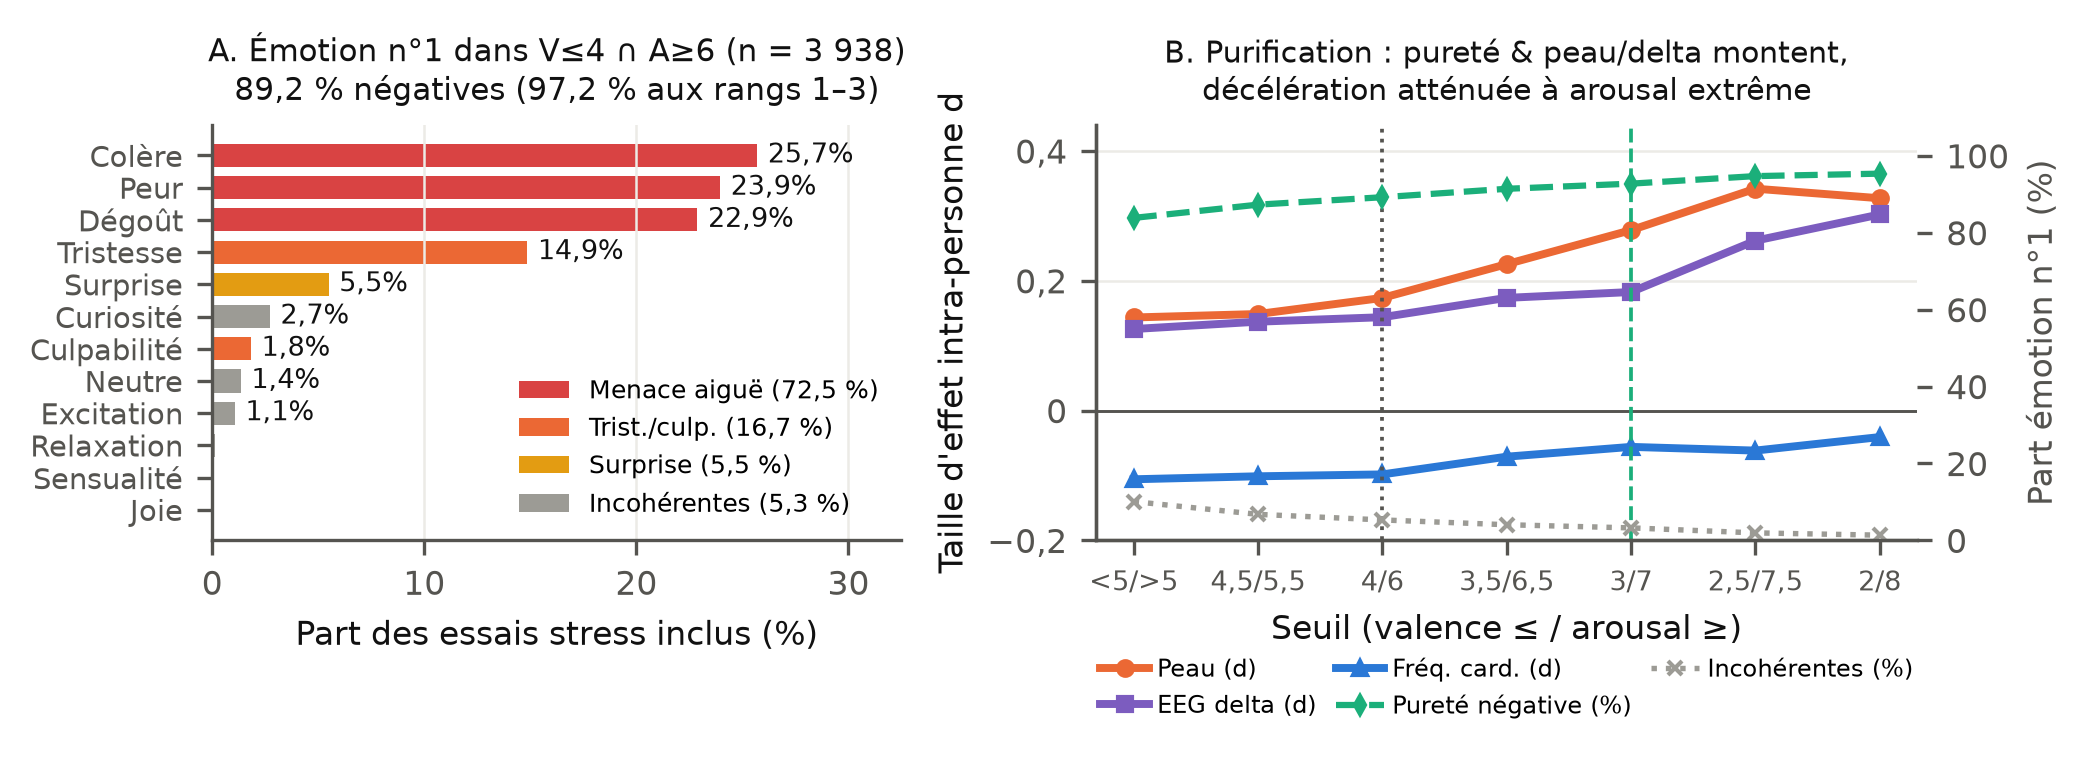
\includegraphics[width=0.92\linewidth]{fig1_criterion_fr.png}\\[-3pt]
{\footnotesize\textbf{Figure 1 --- Audit et purification du critère.} \textbf{A.} 89,2\,\% d'émotions négatives au rang~1 (5,3\,\% d'incohérences) dans $V\le 4 \cap A\ge 6$. \textbf{B.} En durcissant le seuil, peau et delta doublent mais la bradycardie s'atténue aux niveaux d'arousal extrêmes.}
\end{center}

\clearpage

\begin{center}
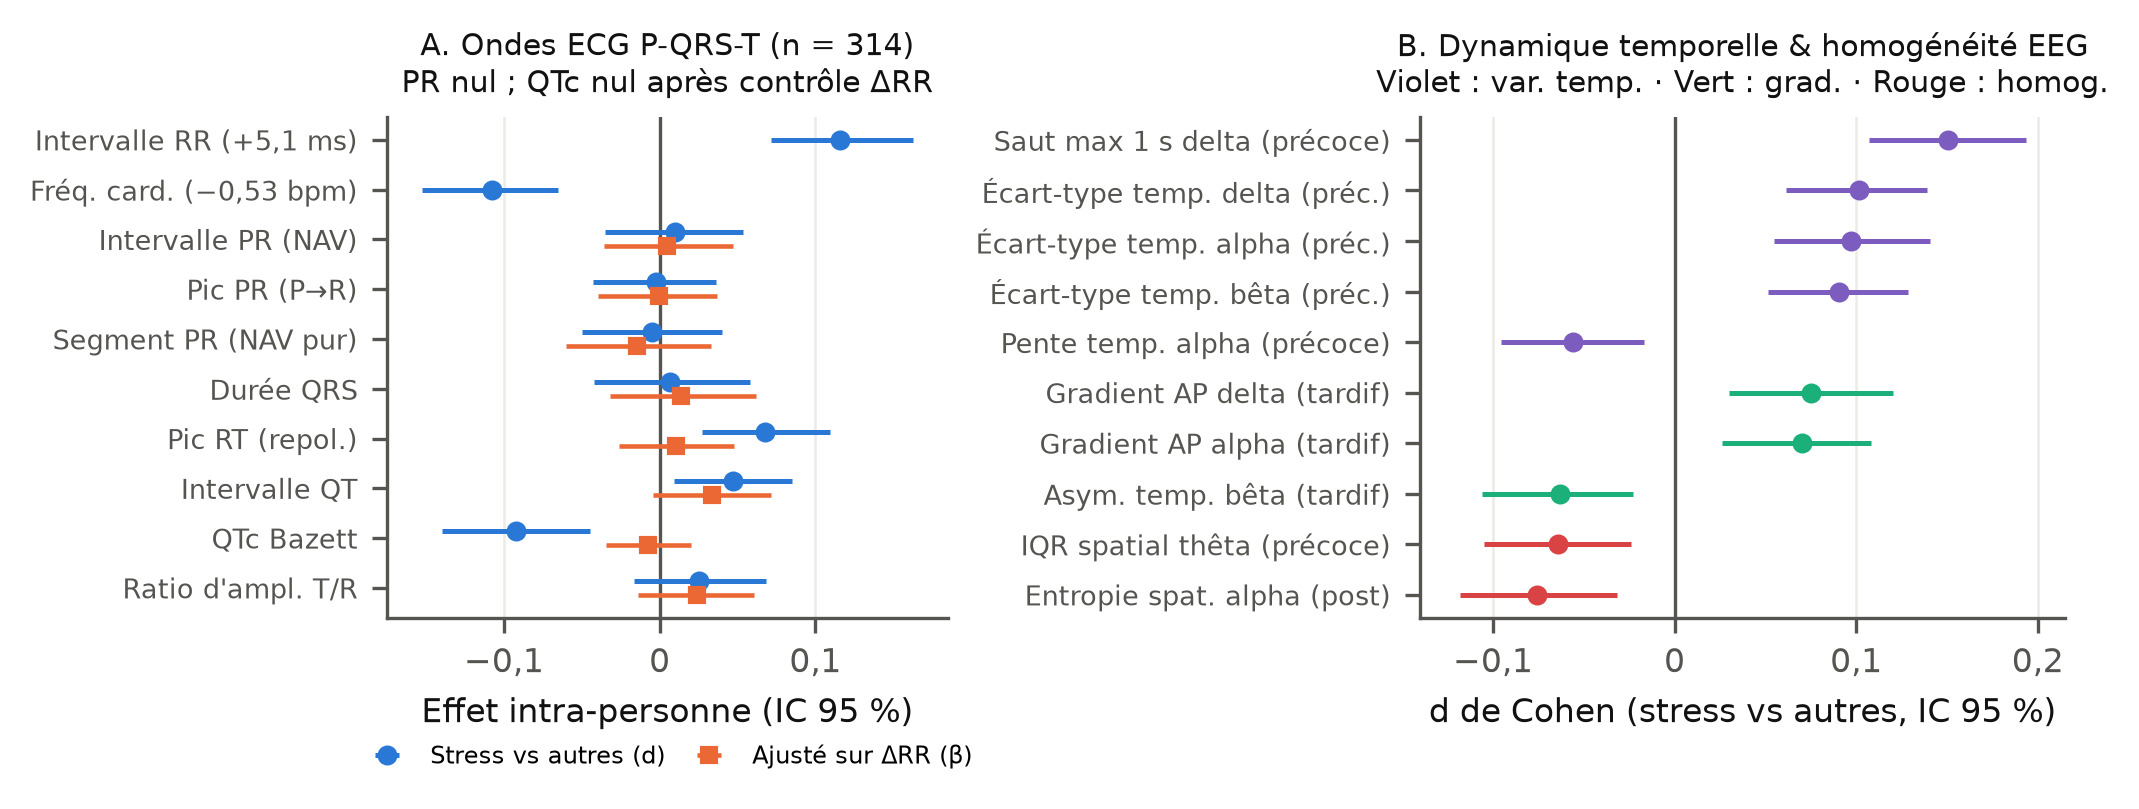
\includegraphics[width=0.84\linewidth]{fig3_ecg_eeg_rich_fr.png}\\[-3pt]
{\footnotesize\textbf{Figure 2 --- Morphologie ECG P-QRS-T et nouvelles dynamiques EEG.} \textbf{A.} RR s'allonge ($+5{,}1$~ms), PR/QRS/T sont nuls, et QTc Bazett s'annule totalement après contrôle $\Delta\mathrm{RR}$ (orange). \textbf{B.} Volatilité temporelle EEG précoce forte (saut $\delta$ : $+0{,}151$) et focalisation spatiale tardive/post.}

\smallskip
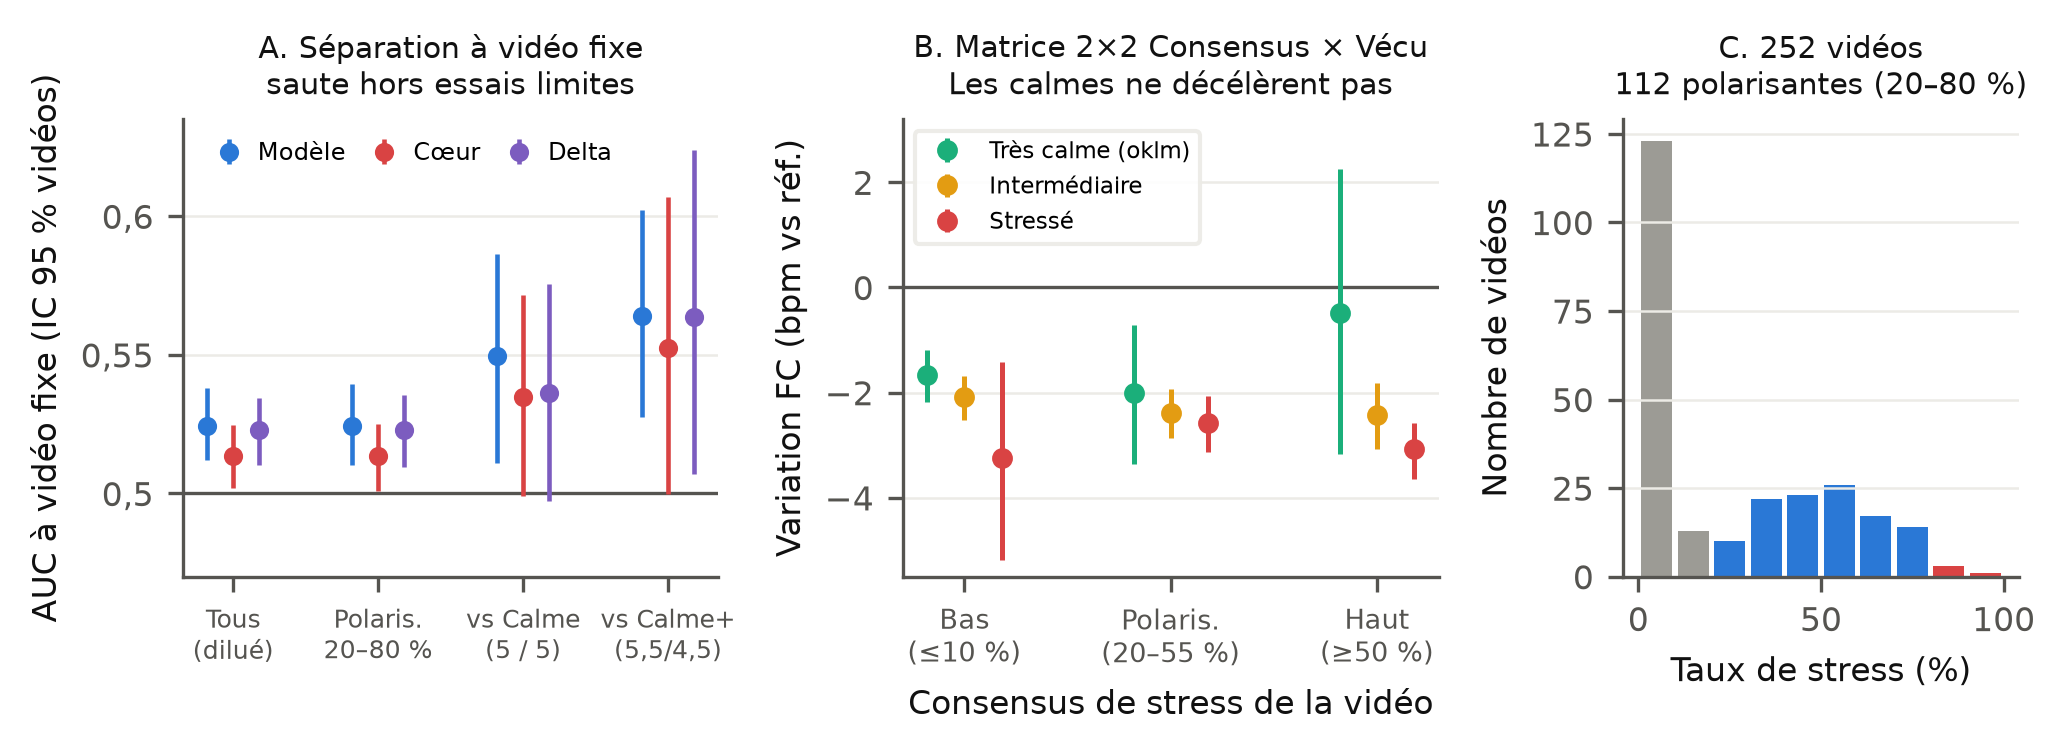
\includegraphics[width=0.84\linewidth]{fig5_fixed_video_fr.png}\\[-3pt]
{\footnotesize\textbf{Figure 3 --- Contraste non adjacent à vidéo fixe et matrice $2\times 2$.} \textbf{A.} Exclure les essais limites fait passer l'AUC à vidéo fixe de 0,525 à 0,564. \textbf{B.} Sur vidéos stressantes, les spectateurs calmes (\og oklm \fg{}) ne montrent aucune bradycardie ($-0{,}49$~bpm) ni réponse cutanée.}
\end{center}

\smallskip
{\small\textbf{Modèle neurophysiologique en trois branches du stress aigu bref}
\begin{enumerate}
\item \textbf{Branche attentionnelle automatique (liée au stimulus) :} la désynchronisation alpha pariéto-occipitale survient même quand le sujet reste parfaitement calme devant une vidéo stressante ($d = -0{,}33$ à $-0{,}41$) ; elle ne distingue donc pas la détresse vécue.
\item \textbf{Branche vagale d'orientation (déclenchée en tout-ou-rien par l'évaluation) :} dès que la vidéo passe sous $V < 5$, la FC ralentit (dès 1~s, $-2{,}4$ à $-3{,}1$~bpm) et la respiration s'amenuise (2~s), sans aucun raccourcissement PR ni changement T --- preuve d'un freinage sinusal vagal sans décharge adrénergique marquée au nœud AV. Chez le spectateur qui reste calme devant le même stimulus, cette bradycardie ne se déclenche pas.
\item \textbf{Branche d'alarme sympathique et corticale (seuil élevé $A \ge 7$) :} la conductance cutanée (dès 4~s) et le delta centro-pariétal doublent, les rythmes rapides frontaux $\beta/\gamma$ reflètent la sensibilité individuelle, et un recrutement sympathique cardiaque commence à contrer la bradycardie (courbe en U à $A = 8$--$9$).
\end{enumerate}

\textbf{Enseignements méthodologiques pour la détection et le monitorage clinique}
\begin{itemize}
\item \textbf{Les 4 phases + EEG riche transforment la généralisation :} remplacer les bins 1~s ($p=340$) par 4 phases ($p=114$) + volatilité/homogénéité EEG + supervision continue Ridge V\&A ou convolutions 1D fait passer l'AUC sur personnes \emph{et} thèmes inédits de 0,526 [0,481 ; 0,570] à \textbf{0,589 [0,540 ; 0,635]} (Ridge : 0,586 ; sujets inédits 0,607 ; 0,656 contre relaxé). Les ondes ECG P-QRS-T n'ajoutent aucun gain sur 10~s, et GBDT/MLP sur-apprennent sur thèmes vus.
\item \textbf{Pièges à éviter :} RMSSD sur 10~s non fiable ($r_{\text{intra}} = 0{,}22$--$0{,}43$) ; QTc Bazett biaisé par la variation rapide de RR ; polarité ECG inversée sur 96,6\,\% des essais HABS ; décalage d'intercept en CV par thèmes sans \texttt{class\_weight="balanced"} ; HEP limité par $\approx 13$ battements/essai.
\item \textbf{Plafond essai par essai :} une AUC de 0,56--0,61 sur un clip isolé de 10~s reste insuffisante pour une décision clinique unitaire ; l'agrégation multi-épisodes et la calibration basale (FC et gamma de repos) sont indispensables.
\end{itemize}

\textbf{Limites et pistes prioritaires pour la revue de littérature}
\begin{itemize}
\item \textbf{Limites :} vidéos passives de 10~s chez l'adulte sain (une douleur aiguë pédiatrique ou un stress prolongé recrute davantage la tachycardie sympathique et potentiellement le segment PR au-delà de 10--30~s) ; 1 seule dérivation ECG ; cellule extrême \og calme sur vidéo stressante \fg{} réduite ($n = 63$) ; possible micro-EMG crânien résiduel dans $\beta/\gamma$ préfrontal malgré l'ICA (contrairement au delta centro-pariétal, validé hors clignement).
\item \textbf{Pistes bibliographiques à croiser ensemble :} (1)~bradycardie vagale d'orientation / \emph{freezing} vs tachycardie nociceptive et délai dromotrope PR ; (2)~hypervigilance anxieuse, tonus gamma préfrontal et FC basale ; (3)~biomarqueurs EEG/SNA en pédiatrie pré-verbale, coma et anesthésie générale ; (4)~protocoles de validation à stimulus fixe non adjacent.
\end{itemize}}

\smallskip
{\footnotesize Article complet (14 pages FR / 13 pages EN), 6 figures haute résolution, protocoles figés et code : \url{https://github.com/mathiaschebbah/habs}}

\end{document}
